\section{Meilenstein 4: 03.07.2019 - 07.08.2019}
Der vierte Meilenstein hat das übergeordnete Ziel, das Produktivsystem aufzusetzen und so quasi die erste Version unseres Systems zu veröffentlichen.
Neben dem Aufsetzen des Produktivsystems sollen zudem weitere Anforderungen umgesetzt werden, die vor allem Features für die jeweiligen Endnutzer (also UIS"=Nutzer und Navigationsnutzer) beinhalten.
In Hinblick auf die beschränkte Restdauer der Projektgruppe wurden daher Anforderungen niedriger priorisiert, die zum Beispiel den Umgang mit der IoT"=Plattform erleichtern oder Ähnliches.
Die Priorisierung der noch bis zum Projektende geplanten Features wurde innerhalb der Umsetzung des Meilensteins mit den Stakeholdern abgestimmt.


In der Vorbereitung des Meilensteins werden daher Szenarien geplant, die mit Abschluss des Meilensteins in Form einer Demo gezeigt werden sollen.
Insgesamt gibt es vier verschiedene Szenarien: Das erste Szenario ist bezogen auf den Navigationsnutzer und beginnt damit, dass der Nutzer einen Start- und Endpunkt in der Navigationsapplikation sowie als Fahrzeug ein Auto auswählen kann.
Nach der Planung der Route werden mehrere Routen vorgeschlagen, welche die vorher festgelegten Parameter erfüllen.
Daraufhin soll der Navigationsnutzer in der Lage sein, nicht die erst ausgewählte (beste) Route zu nehmen, sondern eine der alternativen Routen.
Dann soll der Navigationsnutzer die Navigation starten und abbrechen können.
Das zweite Szenario bezieht sich auch auf den Navigationsnutzer und ist ähnlich aufgebaut das erste Szenario.
Der Unterschied besteht darin, dass unterschiedliche Parameter ausgewählt werden, wie beispielsweise als Fahrzeug ein Fahrrad und die Wahl der besten Route.
Zudem soll eine tatsächliche Navigation stattfinden, indem zum jeweiligen Standort des Navigationsnutzer die entsprechende Navigationsanweisung anzeigt und die bereits zurückgelegte Strecke eingefärbt wird.
Weiterhin wird bei der Abweichung von der verfolgten Route auf die Abweichung hingewiesen.
Das dritte Szenario beinhaltet hauptsächlich das Anzeigen von Zeitreihen zu einem bestimmten Sensorknoten.
Um dies zu ermöglichen, müssen zunächst alle Sensorknoten auf einer Karte angezeigt werden und auch auswählbar sein.
In einer Sidebar werden dann detaillierte Informationen zum Sensorknoten angezeigt, sowie die Möglichkeit geboten, Zeitreihen anzuzeigen
 Neben den Zeitreihen soll zudem eine Heatmap in der Karte angezeigt werden, welche die Feinstaubwerte kategorisiert und so die Belastung in Oldenburg sichtbarer macht.
Das vierte und letzte Szenario richtet sich an Projektinteressierte.
Auf der UIS"=Webseite wird erläutert, wie interessierte Personen einen Sensorknoten selber kaufen, aufbauen, einrichten und montieren können, sodass diese Sensorknoten an unsere IoT"=Plattform senden.


Zusammenfassend zu vierten Meilenstein lässt sich festhalten, dass alle funktionalen Anforderungen umgesetzt werden konnten.
Jedoch besteht an einigen Stellen noch Verbesserungsbedarf.
Dies zeigt sich auch in \Fig{bigpicture3}, in welchem wieder die Erreichung der Ziele in den einzelnen Teilprojekten dargestellt ist.
Verbesserungsbedarf besteht zum Beispiel in den Schnittstellen des UIS"=Frontend zur IoT"=Plattform.

\begin{figure}[!htb]
	\centering
	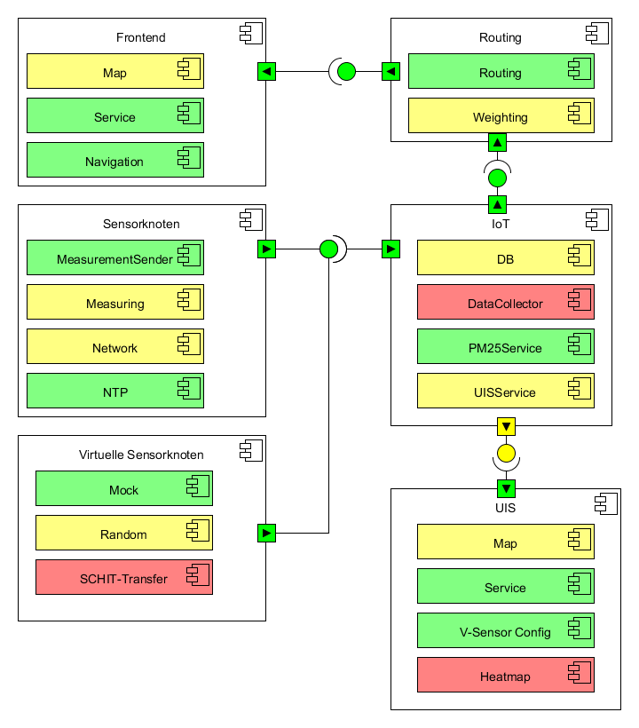
\includegraphics[width=\textwidth]{./ressourcen/bigpicture3.png}
	\caption{Big Picture des vierten Meilensteins}
	\label{fig:bigpicture3}
\end{figure}

So dauert zum Beispiel das Abfragen der Zeitreihendaten eines Sensorknoten bis zu 30 Sekunden.
Neben diesem Umstand gibt es weitere kleinere Fehler, die bis zum Abschluss der Projektgruppe gefixt werden sollten.
Um das System letztendlich robuster zu gestalten, wird in den nächsten Phasen der Projektgruppe der Aspekt des Testens intensiver fokussiert.
Weiterhin sollen diverse weitere Features umgesetzt werden, wie zum Beispiel der Export der Daten eines Sensorknotens.
Zudem soll eine Oberfläche für die Verwaltung von Sensorknoten geschaffen werden und ein Installationstool, welches es Projektinteressierten ermöglicht, die aktuellste Firmware der Projektgruppe auf dem selbst bereitgestellten Sensorknoten zu flashen.
Der dritte Meilenstein zeigt aber insgesamt, dass die Planung und Zusammenarbeit der Projektgruppe immer gezielter und somit auch besser wird.
Dies spiegelt sich insbesondere darin wieder, dass es nur noch weniger Themen gibt, die im Meilenstein gar nicht angegangen worden sind.
Zudem sind die Themen, die in \Fig{bigpicture3} nicht vollständig umgesetzt wurden, oft nahezu fertig und es fehlen noch Kleinigkeiten, wie beispielsweise Unit Tests oder die Entwicklerdokumentation.